%% This is LLNCS.DEM the demonstration file of
% the LaTeX macro package from Springer-Verlag
% for Lecture Notes in Computer Science,
% version 2.4 for LaTeX2e as of 16. April 2010
%
\documentclass{article}

\usepackage[utf8]{inputenc}
\usepackage[top=2.5cm, bottom=2.5cm, left=2cm, right=2cm]{geometry}
\usepackage{graphicx}
\usepackage{color}
\usepackage{float}
\usepackage[small,bf]{caption}
\setlength{\captionmargin}{3pt}
\usepackage{multicol}
\usepackage{blindtext}
\usepackage{geometry}
\usepackage{subfigure}
\usepackage{enumerate}
\usepackage{scalefnt}
\providecommand{\keywords}[1]{\textbf{\textit{Keywords:}} #1}
%
%
\begin{document}

%
%
% ------------------------------------------------------------

\title{Urban Street Networks, a comparative study of Portuguese cities}
%
\author{Bruno Casteleiro\\
	{\texttt{(up201505347@fc.up.pt)}}\\
	\multicolumn{1}{p{.7\textwidth}}{\centering\emph{
		\\Departamento de Ciências de Computadores,\\Faculdade de Ciências da Universidade do Porto}}
}

\date{\today}

\maketitle

% ------------------------------------------------------------

%----------------------ABSTRACT----------------------%

\begin{abstract}
\vspace{3mm}
\keywords{Graphs, complex network, graph theory, nodes, edges, Gephi, OSM, city, Portugal}
\vspace{5mm}
\end{abstract}

% ------------------------------------------------------------

\begin{multicols}{2}

%----------------------INTRODUCTION----------------------%

\section{Introduction}

%----------------------DATA COLLECTION AND PROCESSING----------------------%

\section{Data Collection and Processing}
\label{section.data}

As in any network study, having data, and a source to get it, is essential. In an optimal scenario, the choosed data source provides not only complete information to work with, but also correct information. Although heavily relieing on crowd-sourcing - thus having some inconsistency here and that -, we found OpenStreetMap (OSM) to be a sufficiently robust and well formatted data source to use for this study. 

To make the process of downloading data from OSM easier, the Overpass API was used. Overpass "acts as a database over the web" for OSM, and give us the possibility to query for data in a variant of the so desired JSON format, the Overpass JSON. With this, its was only necessary to create a file with the many city's boundary box coordinates and pass it as input to our download script, which then processed it and download OSM data using the API.

Having downloaded every city's OSM data, its then only necessary to create the corresponding Network. To OSM, streets are considered "ways", collections of ordered nodes and some tags detailing the street.  Moreover, nodes also contains important information such as its latitude and longitude. Since we wanted to study the cities in their primal form, thus preserving its geographical properties, our parse algorithm simply convert each OSM node into a graph node and each OSM way in edges that connect sequentially from node to node. Nodes and edges are finally saved in different csv files.

Each network is then imported to Gephi where we can visualize and analyse it.


%----------------------FIGURES 1 AND 2----------------------%

\begin{figure*}[ht]
\begin{minipage}[b]{0.5\linewidth}
\centering
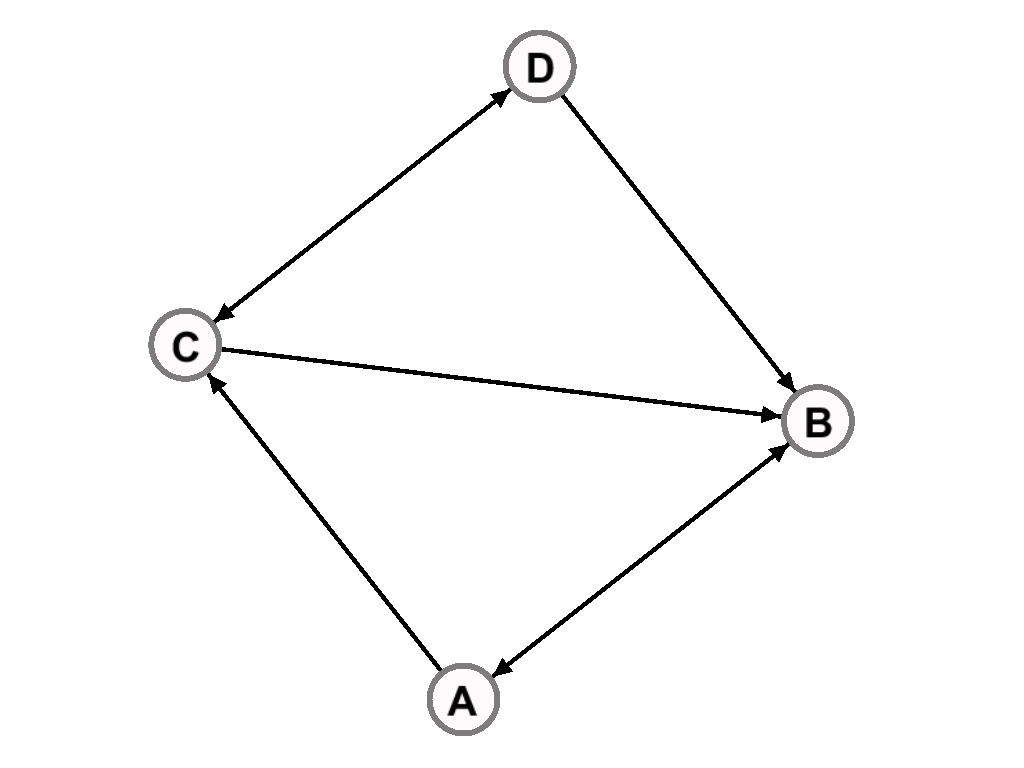
\includegraphics[width=5.5cm,height=4cm]{Figures/graph_directed}
\caption{Directed graph (digraph).}
\label{fig:figure1}
\end{minipage}
\hspace{0.5cm}
\begin{minipage}[b]{0.4\linewidth}
\centering
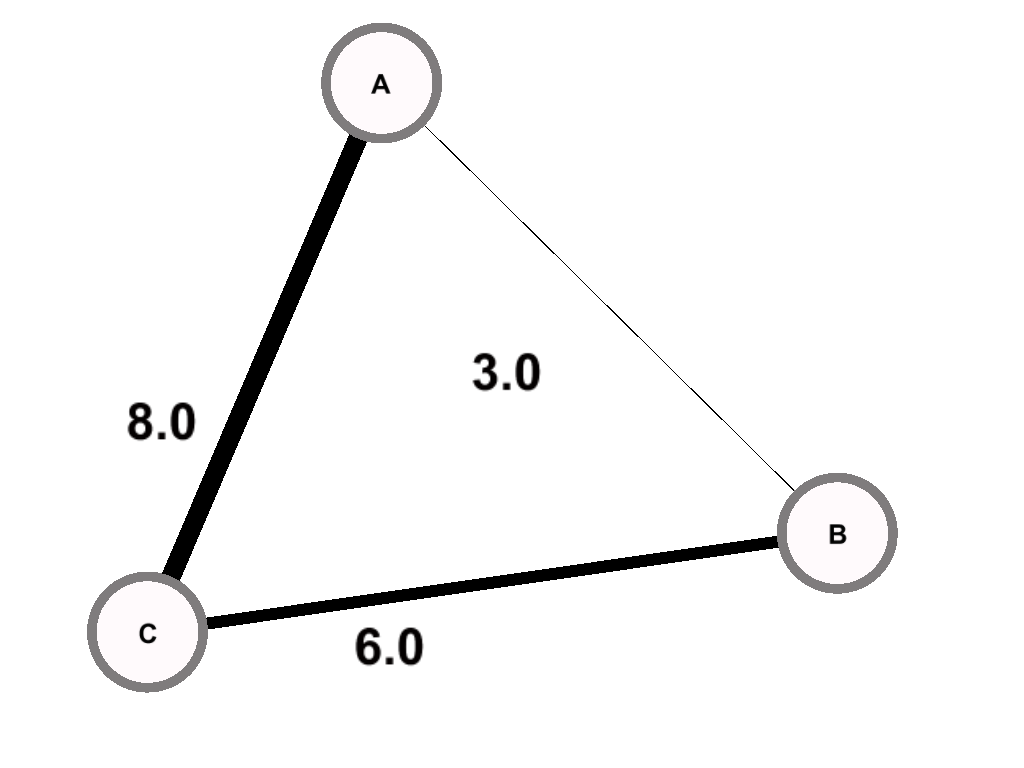
\includegraphics[width=5.5cm,height=4cm]{Figures/graph_undirected_weighted}
\caption{Weighted undirected graph.}
\label{fig:figure2}
\end{minipage}
\end{figure*}


%----------------------ANALYSIS AND RESULTS----------------------%

\section{Analysis and Results}
\label{section.results}


\section{Conclusion}
\label{section.conclusions}


% ------------------------------------------------------------

\bibliographystyle{splncs03}
\bibliography{report}
\end{multicols}
\end{document}
